%%%%%%%%%%%%%%%%%%%%%%%%%%%%%%%%%%%%%%%%%%%%%%%%%%%%%%%%%%%%%%%%%%%%%%%%%%%%%%%%%%%
\subsection{Representação eficiente de formas}
%%%%%%%%%%%%%%%%%%%%%%%%%%%%%%%%%%%%%%%%%%%%%%%%%%%%%%%%%%%%%%%%%%%%%%%%%%%%%%%%%%%

%%%%%%%%%%%%%%%%%%%%%%%%%%%%% SLIDE 4.0 %%%%%%%%%%%%%%%%%%%%%%%%%%%%%%%%%%%%%%%%%%%
\begin{frame}
\frametitle{{\bf \color{blue} Aplicações}}
	
\begin{block}{\bf Representação eficiente de formas}
Se utilizada uma boa base para representação, é necessária apenas uma parcela da função de base para representar toda a geometria.
\end{block}

\begin{center}
	\begin{figure}
	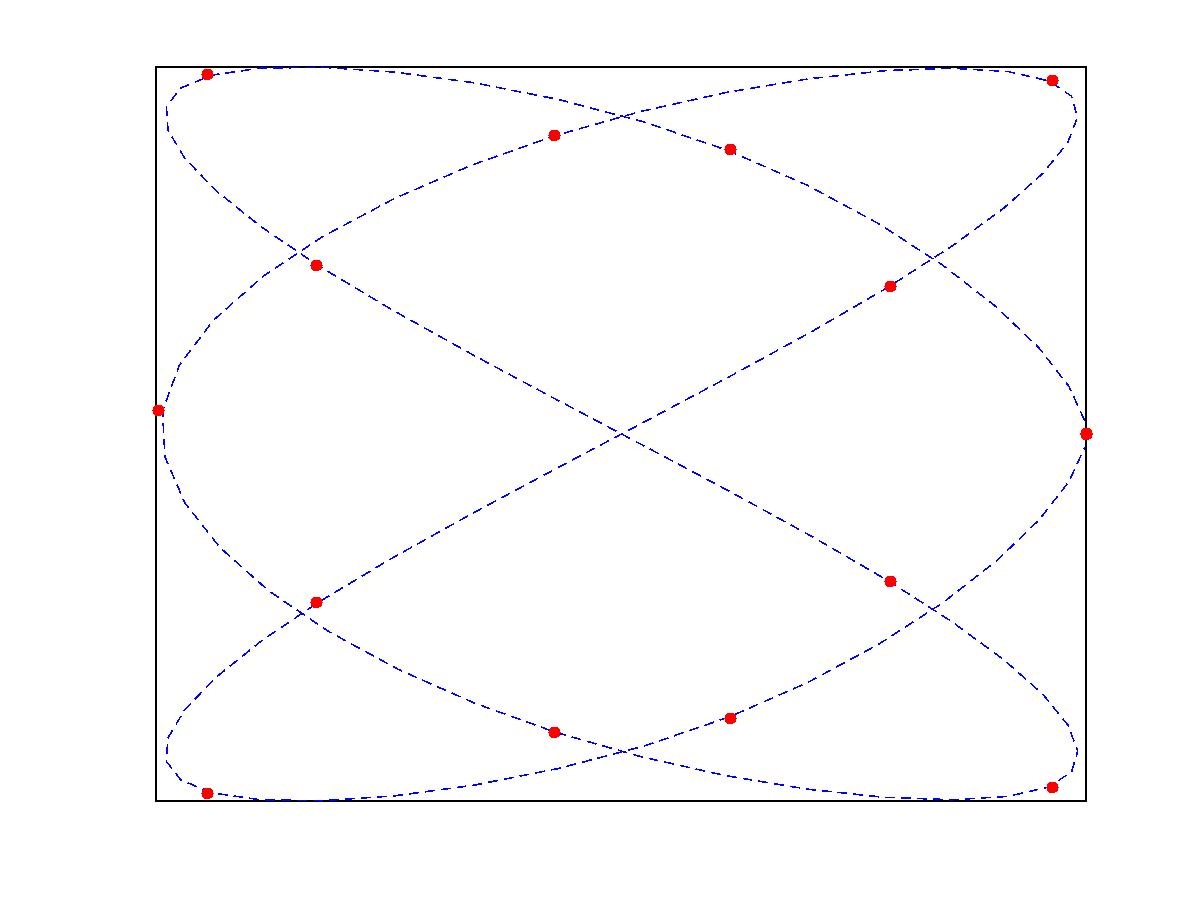
\includegraphics[trim={4cm, 3cm, 4cm, 2cm},clip,width=0.4\linewidth]{imagens/rep_dashed.jpg}
	\caption{Função paramétrica estimada a partir dos pontos em vermelho (âncora) e de informações de conectividade da malha.}
	\end{figure}
\end{center}
	
\end{frame}

\begin{frame}
\frametitle{{\bf \color{blue} Aplicações}}
\framesubtitle{\color{blue} Representação eficiente de formas}
	
	\begin{block}{\bf Representação eficiente de formas}
		Com apenas informações de conectividade da malha e alguns pontos fixados (denominados vértices âncora), é possível aproximar toda a geometria, a partir da resolução do sistema pelo método dos mínimos quadrados:
		
		\begin{equation}\label{eq:sisrecover}
			\left( \frac{L}{\omega I_{m \times m} | 0} \right) \mathbf{x'} = \begin{pmatrix}
				0\\
				\omega\ c_{1:m}^{(x)}
			\end{pmatrix}
		\end{equation}
		
		em que $c = \{v_1, v_2, \dots, v_m\}$ são os pontos âncora escolhidos como amostra, e $\omega > 0$ é o peso de cada restrição).
	\end{block}
	
\end{frame}

\begin{frame}
	\frametitle{{\bf \color{blue} Aplicações}}
	\framesubtitle{\color{blue} Representação eficiente de formas}
	
	\begin{block}{\bf Representação eficiente de formas}
		Graficamente, para facilitar a visualização, este sistema matricial também pode ser visto deste jeito:
		
		\begin{center}
			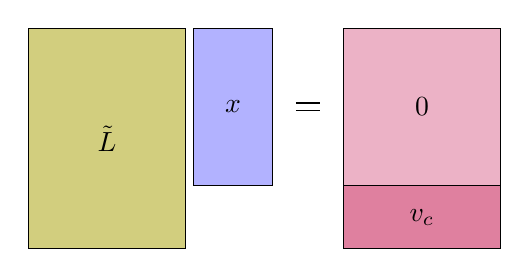
\begin{tikzpicture}
				\filldraw[fill=olive!40!white, draw=black] (0,-0.8) rectangle node{$\tilde{L}$} (2,2);
				\filldraw[fill=blue!30!white, draw=black] (2.1,0) rectangle node{$x$} (3.1,2);
				\draw (3.4, 0.95) -- (3.7, 0.95);
				\draw (3.4, 1.05) -- (3.7, 1.05);
				\filldraw[fill=purple!30!white, draw=black] (4,0) rectangle node{$0$} (6,2);
				\filldraw[fill=purple!50!white, draw=black] (4,0) rectangle node{$v_c$} (6,-0.8);
			\end{tikzpicture}
		\end{center}
		
	\end{block}
	
\end{frame}


\begin{frame}
\frametitle{{\bf \color{blue} Aplicações}}
\framesubtitle{\color{blue} Representação eficiente de formas}
	
\begin{block}{\bf Reconstrução - observações}
Em vez de $\delta^{(x)}$ do lado direito, informa-se $0$ nas coordenadas em que não sabe a localização.

\medskip

Estas localizações serão calculadas por informações das malhas, descritas na matriz $\tilde{L}$.

\medskip

Por isso, é importante que se tenha conhecimento de informações de conectividade da malha em análise.
\end{block}
\end{frame}


\begin{frame}[fragile]
\frametitle{{\bf \color{blue} Aplicações}}
\framesubtitle{\color{blue} Representação eficiente de formas}

\begin{block}{\bf Reconstrução - observações}
Caso se saiba que a malha é, por exemplo, uma curva contínua e fechada no $\mathbb{R}^2$, pode-se utilizar o seguinte código para geração da matriz de adjacências:
\end{block}

\begin{Codigo}[geração de matriz de adjacências]
\noindent\rule{11.2cm}{1.pt}
\vspace{-0.2cm}
\begin{verbatim}
function [ A ] = geraAdjacenciaPadrao(n)
 % Entrada:
 %   n: numero de vertices
 A = zeros(n);
 for i=1:n
   A(i,mod(i-2, n)+1) = 1;
   A(i,mod(i, n)+1) = 1;
 end
end
\end{verbatim}\\
\vspace{-0.5cm}
\noindent\rule{11.2cm}{1.pt}\\
\end{Codigo}
\end{frame}


\begin{frame}[fragile]
\frametitle{{\bf \color{blue} Aplicações}}
\framesubtitle{\color{blue} Representação eficiente de formas}

\begin{Codigo}[reconstrução de curva a partir de poucos pontos]
\noindent\rule{11.2cm}{1.pt}
\vspace{-0.2cm}
\begin{verbatim}
n = 100; % numero de pontos no total
n_coords = 2; % dimensao
t = linspace(0, 2*pi, n); % dominio
v = [cos(t) + sin(t); cos(t)]; % v(x, y)'; % v(x, y)

n_known = 11; % reconstrucao com pontos linearmente espacados
known = round(linspace(1, n, n_known));
v_known = zeros(n, n_coords);
v_known(known,:) = v(known,:);

A = geraAdjacenciaPadrao(n);
Ls = geraLaplaciano(A);
delta = zeros(n, n_coords);
recovered = recuperaCoords(Ls, delta, known, v_known(known,:))
\end{verbatim}\\
\vspace{-0.5cm}
\noindent\rule{11.2cm}{1.pt}\\
\end{Codigo}
\end{frame}


\begin{frame}
\frametitle{{\bf \color{blue} Aplicações}}
\framesubtitle{\color{blue} Representação eficiente de formas}

\begin{figure}
	\centering
	\begin{subfigure}[b]{0.31\textwidth}
		\centering
		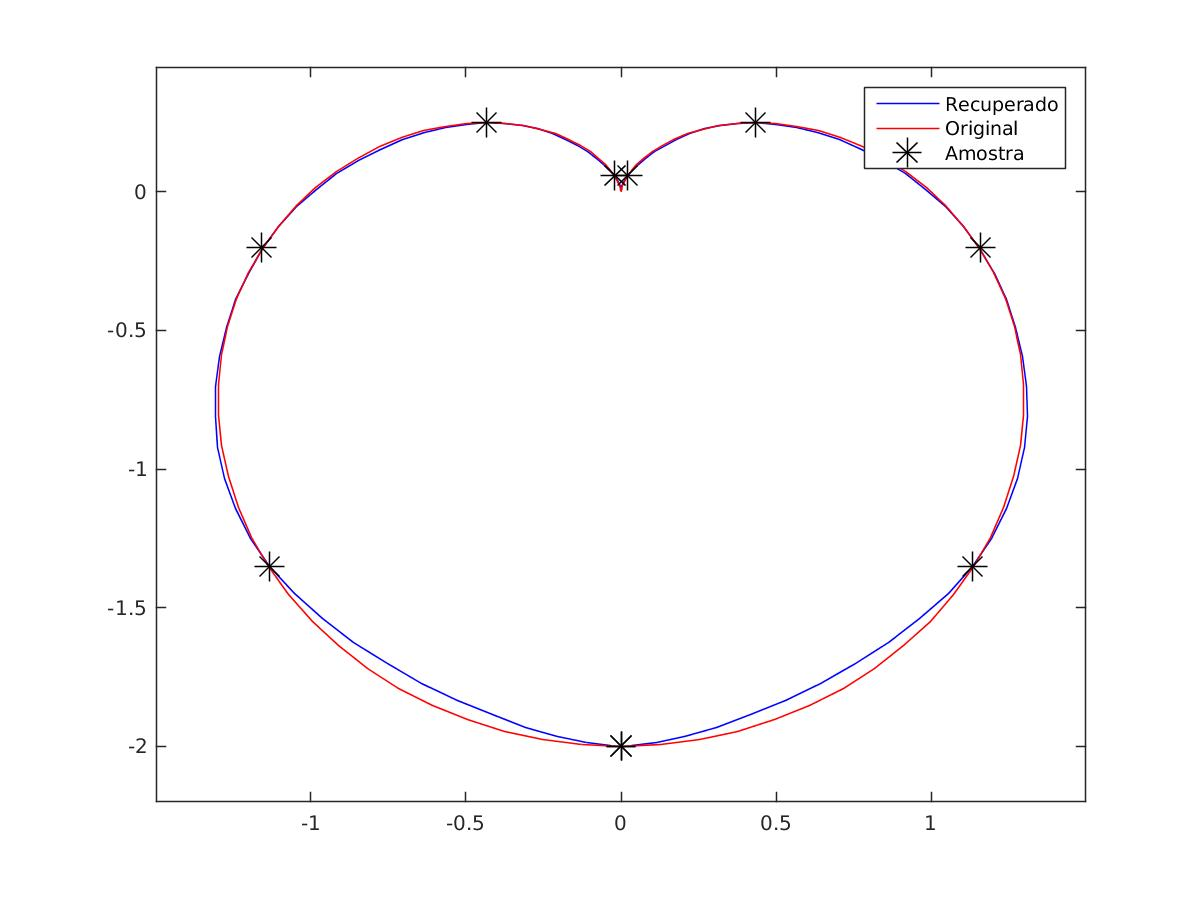
\includegraphics[trim={5cm 2cm 3cm 2cm},clip,width=\textwidth]{imagens/rep_1_10.jpg}
		\caption{10 pontos}
		\label{fig:ex14}
	\end{subfigure}
	\hfill
	\begin{subfigure}[b]{0.31\textwidth}
		\centering
		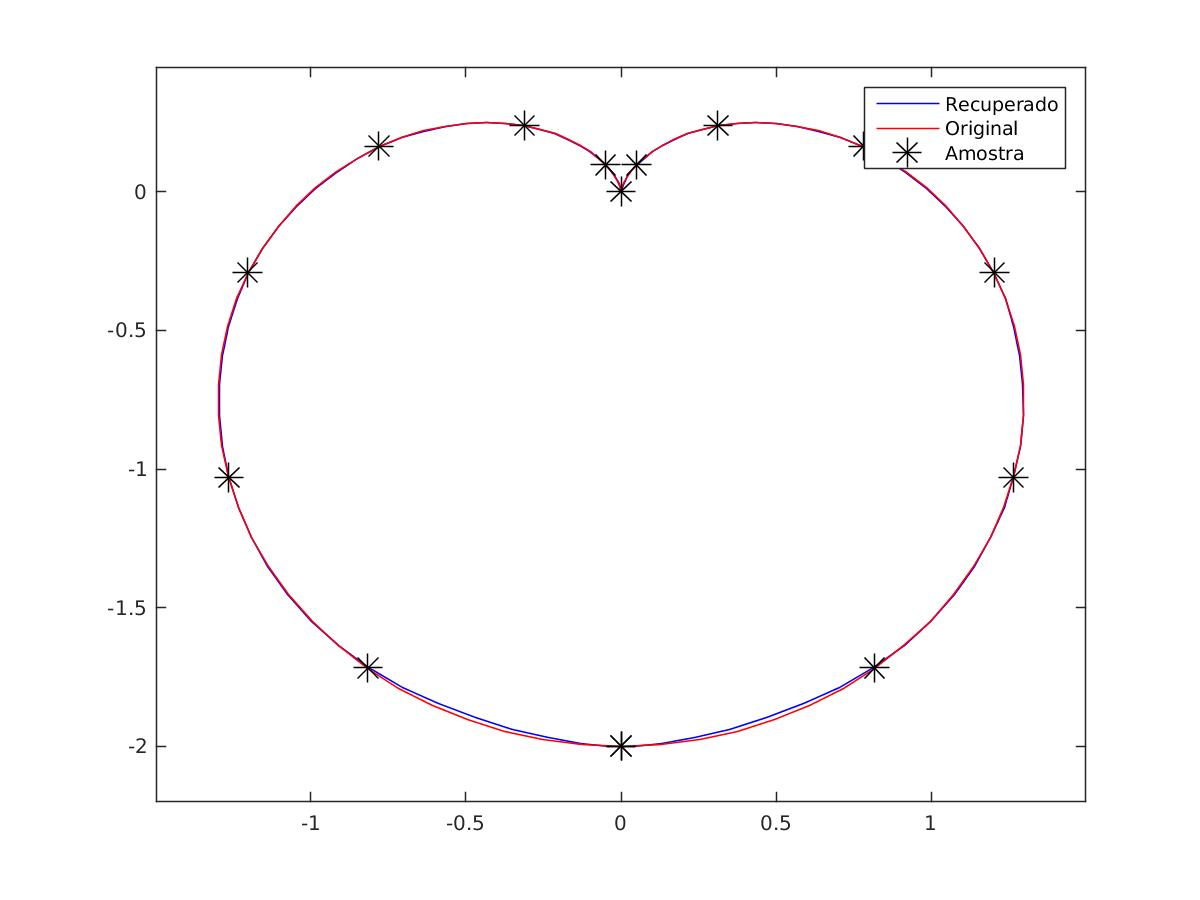
\includegraphics[trim={5cm 2cm 3cm 2cm},clip,width=\textwidth]{imagens/rep_1_15.jpg}
		\caption{15 pontos}
		\label{fig:ex12}
	\end{subfigure}
	\hfill
	\begin{subfigure}[b]{0.31\textwidth}
		\centering
		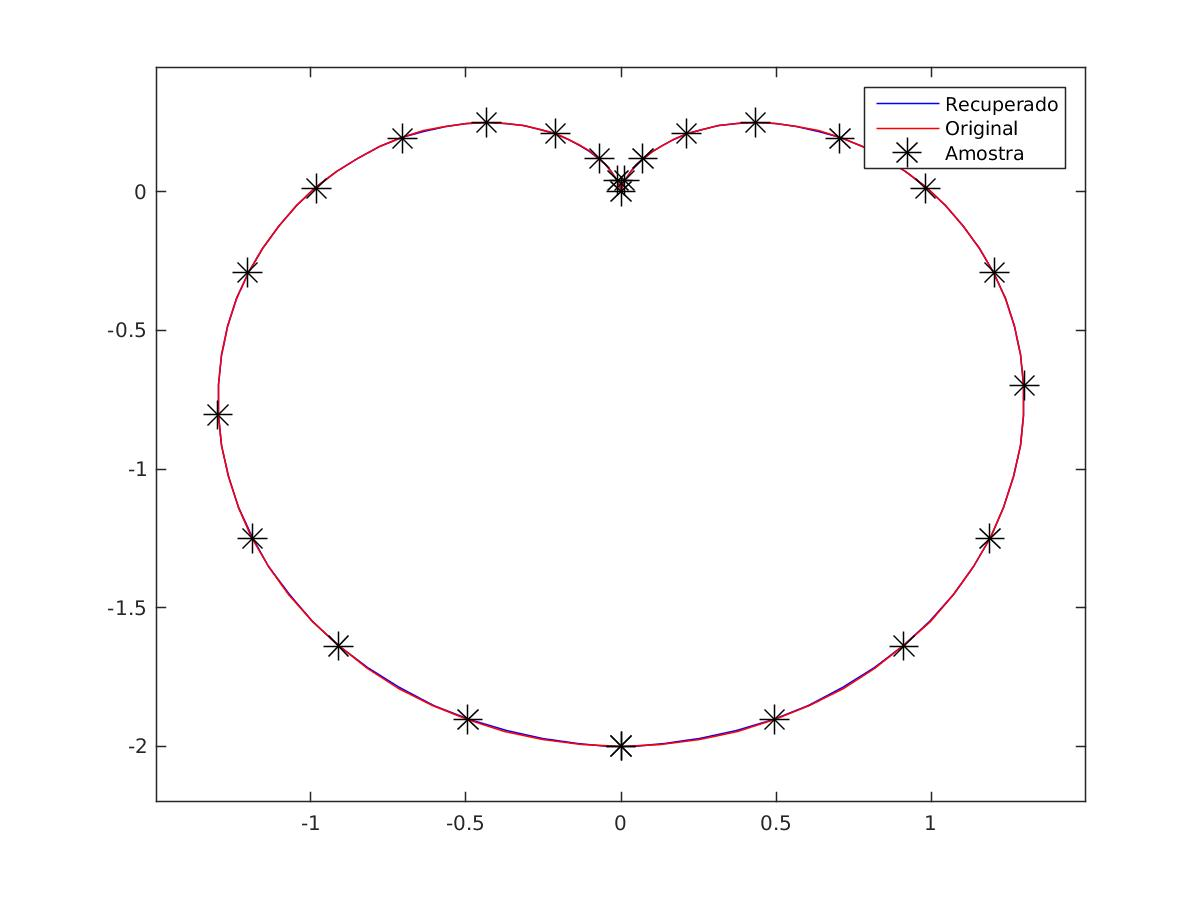
\includegraphics[trim={5cm 2cm 3cm 2cm},clip,width=\textwidth]{imagens/rep_1_25.jpg}
		\caption{25 pontos}
		\label{fig:ex13}
	\end{subfigure}
	\caption{Representação da função paramétrica $(x(t), y(t)) = (sin(t) + 0.5 sen(2t), -cos(t) - 0.5 - 0.5 cos(2t))$ utilizando alguns pontos igualmente espaçados como amostra.}
	\label{fig:ex1rep}
\end{figure}

\end{frame}


\begin{frame}
\frametitle{{\bf \color{blue} Aplicações}}
\framesubtitle{\color{blue} Representação eficiente de formas}

\begin{figure}
	\centering
	\begin{subfigure}[b]{0.31\textwidth}
		\centering
		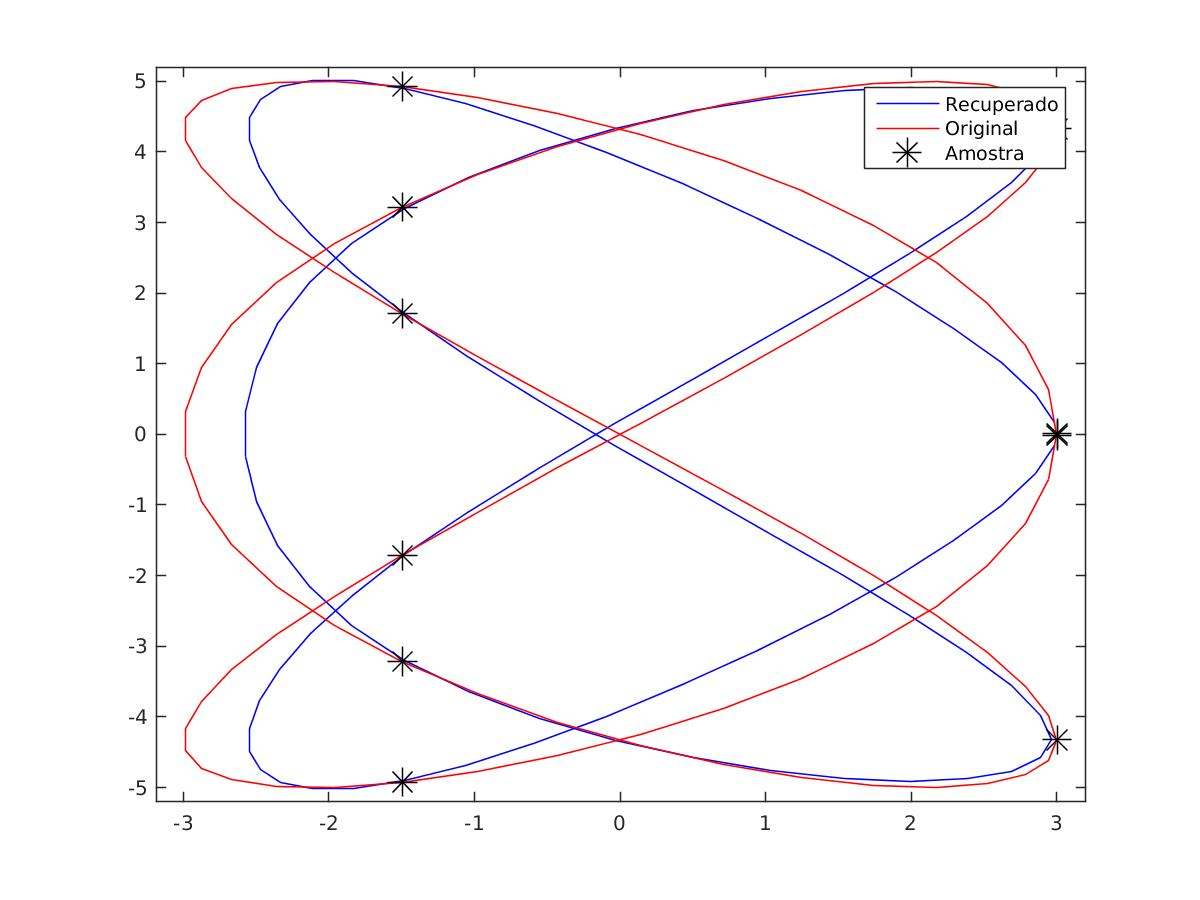
\includegraphics[trim={5cm 2cm 3cm 2cm},clip,width=\textwidth]{imagens/rep_2_10.jpg}
		\caption{10 pontos}
		\label{fig:ex24}
	\end{subfigure}
	\hfill
	\begin{subfigure}[b]{0.31\textwidth}
		\centering
		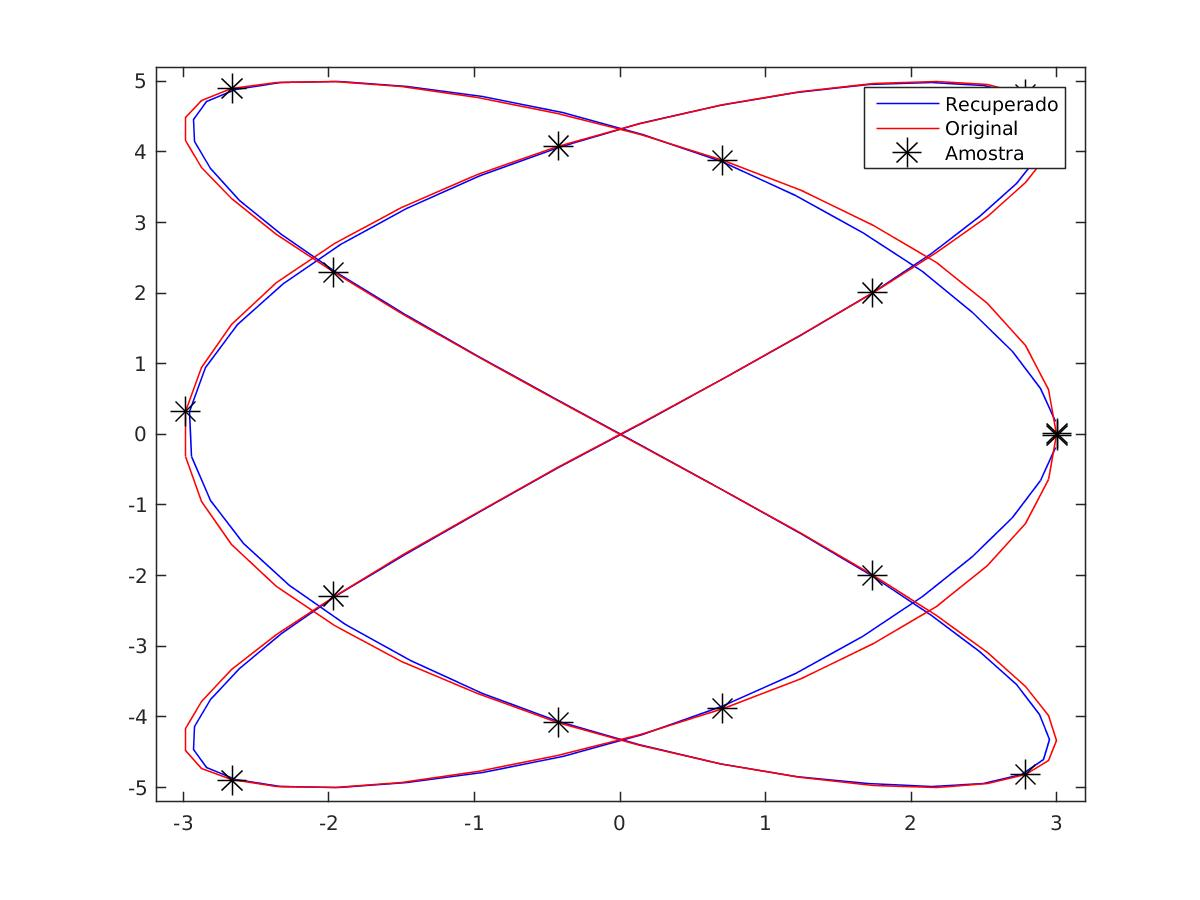
\includegraphics[trim={5cm 2cm 3cm 2cm},clip,width=\textwidth]{imagens/rep_2_15.jpg}
		\caption{15 pontos}
		\label{fig:ex22}
	\end{subfigure}
	\hfill
	\begin{subfigure}[b]{0.31\textwidth}
		\centering
		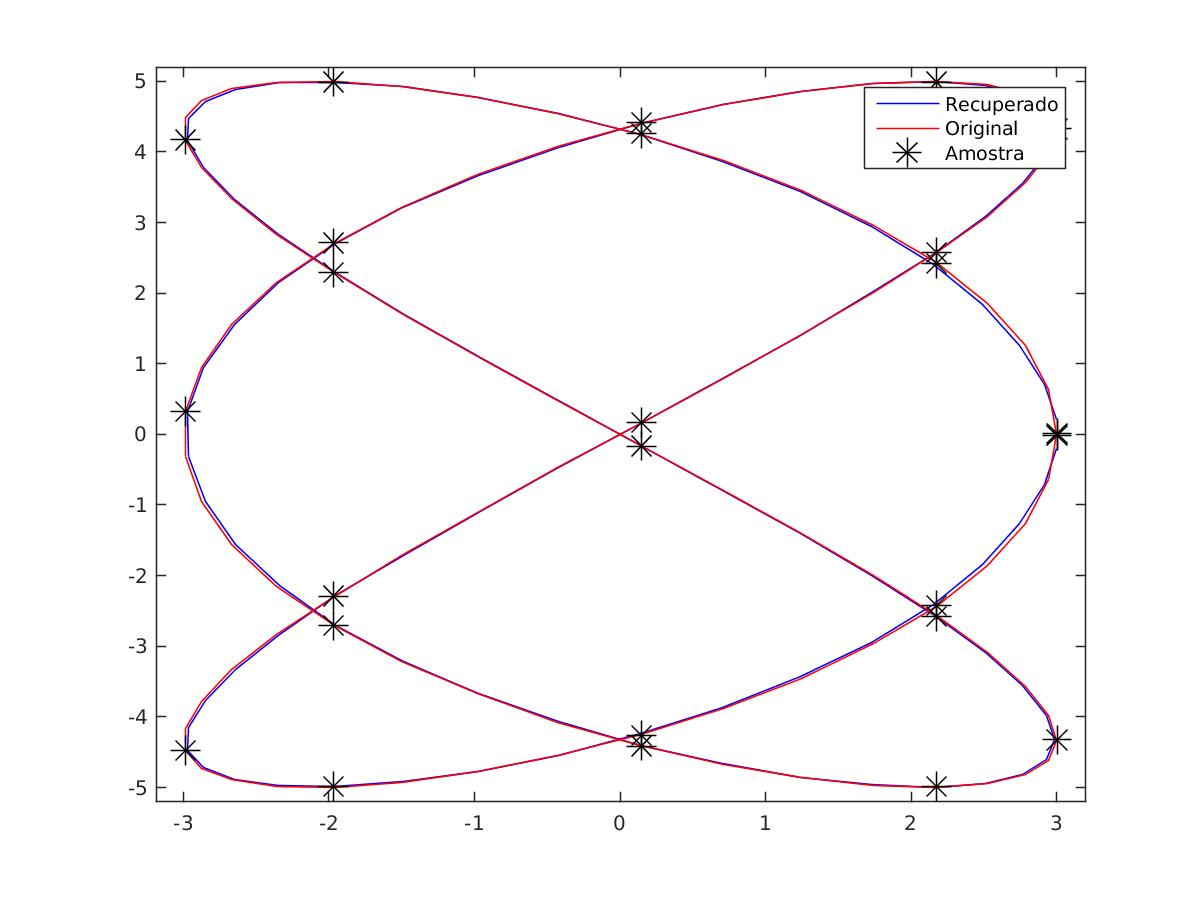
\includegraphics[trim={5cm 2cm 3cm 2cm},clip,width=\textwidth]{imagens/rep_2_25.jpg}
		\caption{25 pontos}
		\label{fig:ex23}
	\end{subfigure} %[3 * cos(3 * t); 5 * sin(2 * t)]';
	\caption{Representação da função paramétrica $(x(t), y(t)) = (3 cos(3t), 5sen(2t))$ utilizando alguns pontos igualmente espaçados como amostra.}
	\label{fig:ex2rep}
\end{figure}


\end{frame}


\begin{frame}
\frametitle{{\bf \color{blue} Aplicações}}
\framesubtitle{\color{blue} Representação eficiente de formas}
	\begin{block}{\bf Reconstrução de superfícies}
		Também é possível representar superfícies lineares por partes a partir de poucas amostras na variedade original.
	\end{block}
	\begin{figure}
		\centering
		\begin{subfigure}[b]{0.49\textwidth}
			\centering
			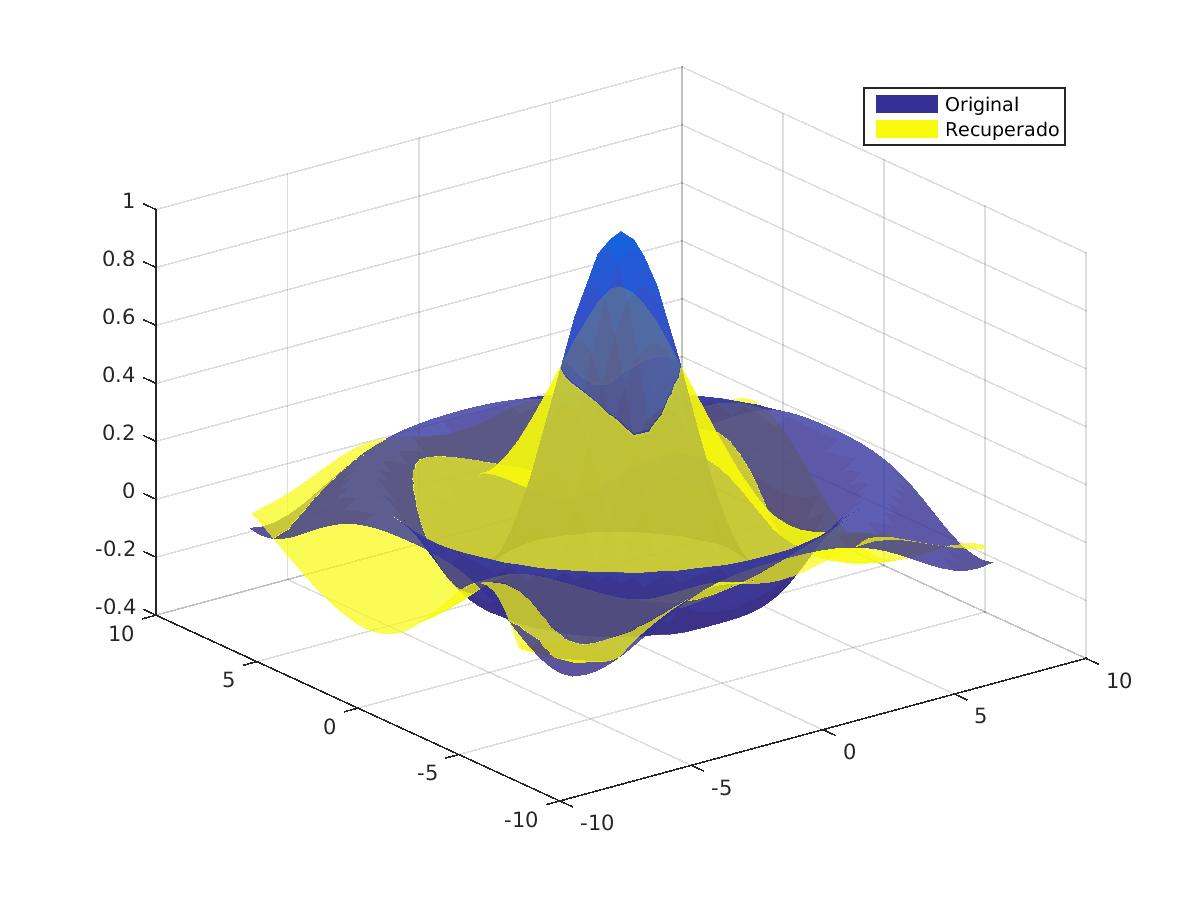
\includegraphics[width=0.9\textwidth]{imagens/rep3_50.jpg}
			\caption{50 pontos}
			\label{fig:surf100}
		\end{subfigure}
		\hfill
		\begin{subfigure}[b]{0.49\textwidth}
			\centering
			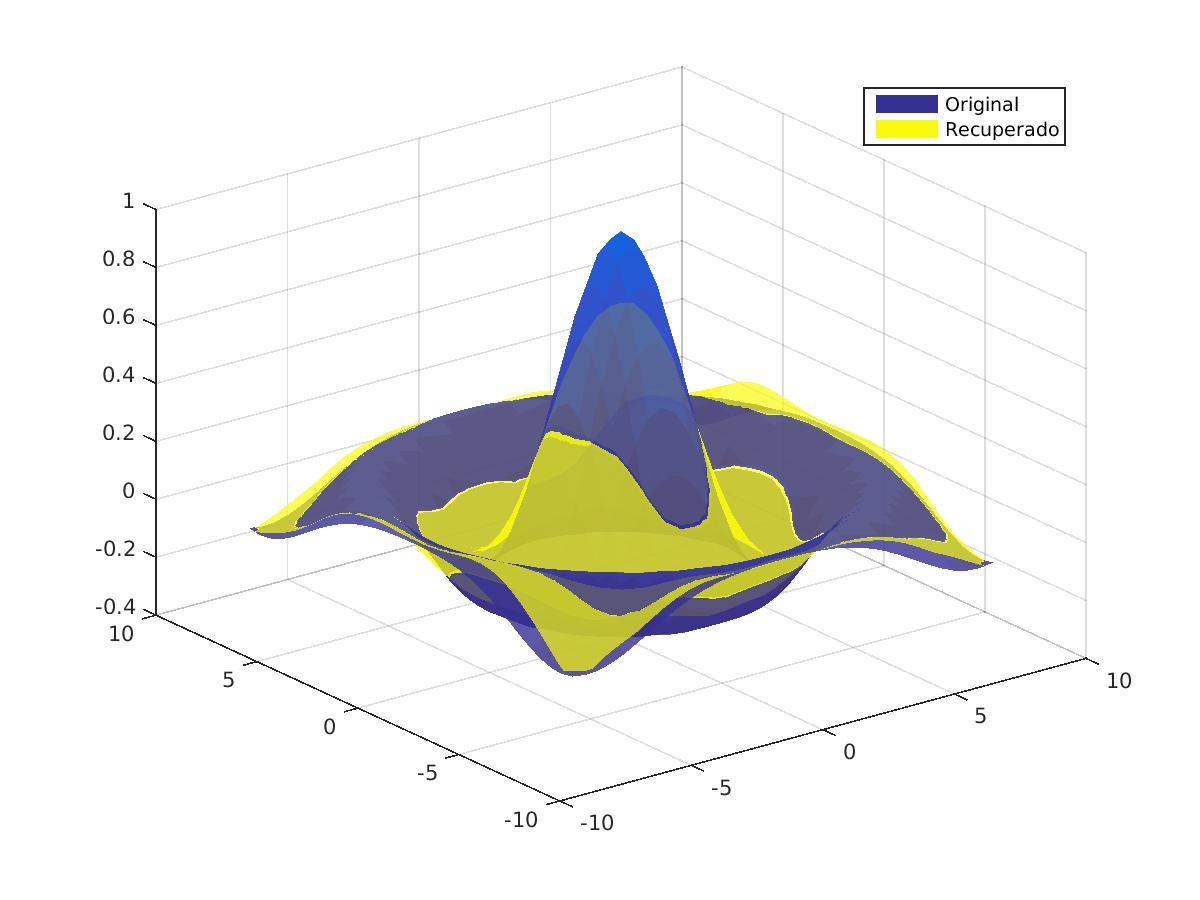
\includegraphics[width=0.9\textwidth]{imagens/rep3_200.jpg}
			\caption{200 pontos}
			\label{fig:surf300}
		\end{subfigure}
		\caption{Reconstrução de superfície utilizando alguns poucos pontos.}
	\end{figure}
	
\end{frame}

%%%%%%%%%%%%%%%%%%%%%%%%%%%%%%%%%%%%%%%%%%%%%%%%%%%%%%%%%%%%%%%%%%%%%%%%%%%%%%%%%%%
\subsection{Edição de malhas e interpolação}
%%%%%%%%%%%%%%%%%%%%%%%%%%%%%%%%%%%%%%%%%%%%%%%%%%%%%%%%%%%%%%%%%%%%%%%%%%%%%%%%%%%

%%%%%%%%%%%%%%%%%%%%%%%%%%%%% SLIDE 4.0 %%%%%%%%%%%%%%%%%%%%%%%%%%%%%%%%%%%%%%%%%%%
\begin{frame}
\frametitle{{\bf \color{blue} Aplicações}}
	
\begin{block}{\bf Edição de malhas}
	Outra interessante aplicação é a de edições de malhas, como movimentos e deformações.
\end{block}

\begin{center}
	\begin{figure}
		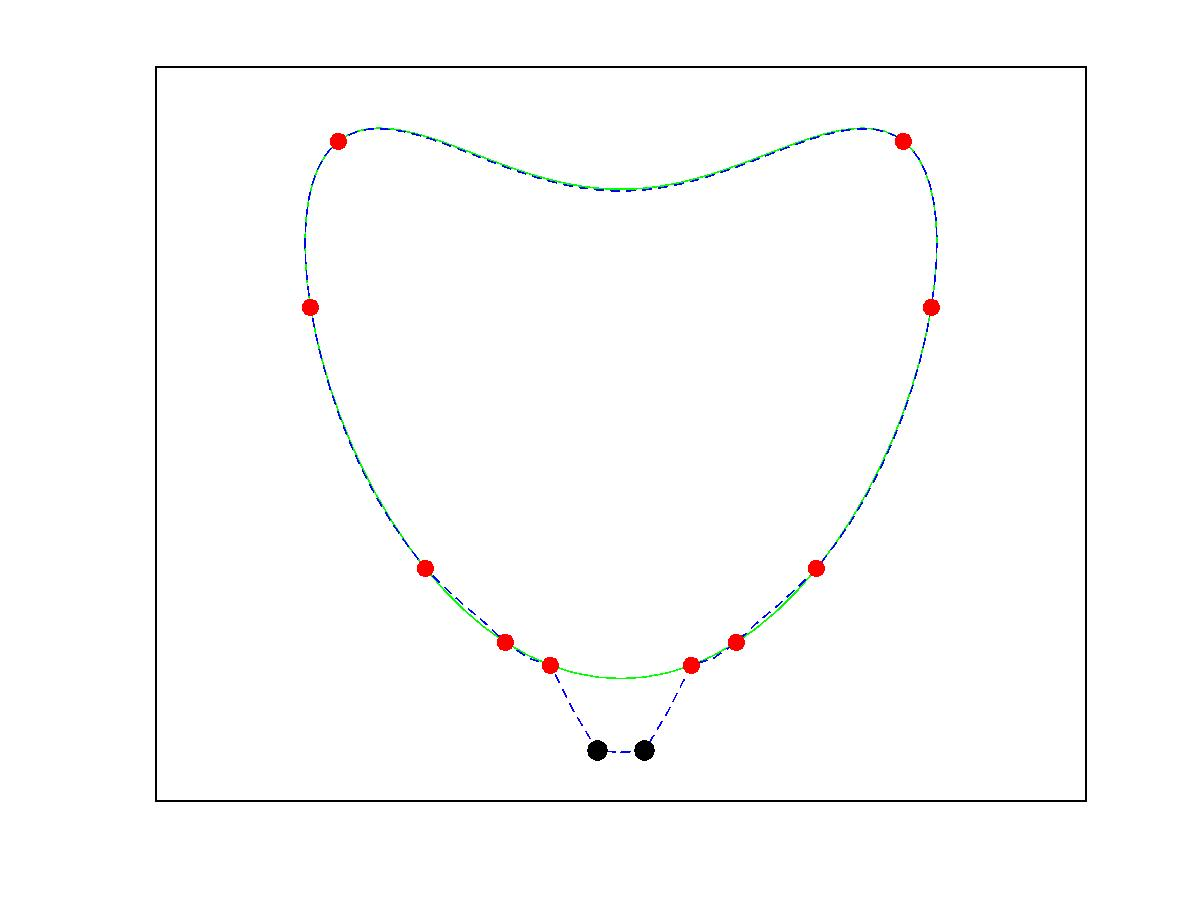
\includegraphics[trim={4cm, 3cm, 4cm, 2cm},clip,width=0.5\linewidth]{imagens/edi_dashed.jpg}
		\caption{Malha original (verde), malha editada (vermelho), pontos âncora (vermelho) e pontos de edição (preto)}
	\end{figure}
\end{center}

\end{frame}

\begin{frame}
	\frametitle{{\bf \color{blue} Aplicações}}
	\framesubtitle{\color{blue} Edição de malhas}
	
	\begin{block}{\bf Edição de malhas}
		Além dos pontos âncoras fixados vistos anteriormente, também são escolhidos alguns pontos de edição, em que se deseja alterar a posição cartesiana, e são adicionadas restrições do tipo:
		
		\begin{align}
			\mathbf{v}_i &= \mathbf{c}_i, &i \in \{1, \dots, m\}\\
			\mathbf{v}_j &= \mathbf{e}_j, &j \in \{m+1, \dots, m+a\}
		\end{align}
		
		\noindent e, matricialmente, o sistema pode ser escrito como:
		
		\begin{equation}\label{eq:sisrecoveredi}
			\left( \frac{L}{\omega I_{(m+a) \times (m+a)} | 0} \right) \mathbf{x'} = \begin{pmatrix}
				\delta^{(x)}\\
				\omega\ c_{1:m}^{(x)}\\
				\omega\ e_{1:a}^{(x)}
			\end{pmatrix}
		\end{equation}
	\end{block}
	
\end{frame}


\begin{frame}
	\frametitle{{\bf \color{blue} Aplicações}}
	\framesubtitle{\color{blue} Edição de malhas}
	
	\begin{block}{\bf Edição de malhas}
		Graficamente, para facilitar a visualização, este sistema matricial também pode ser visto como:
		
		\begin{center}
		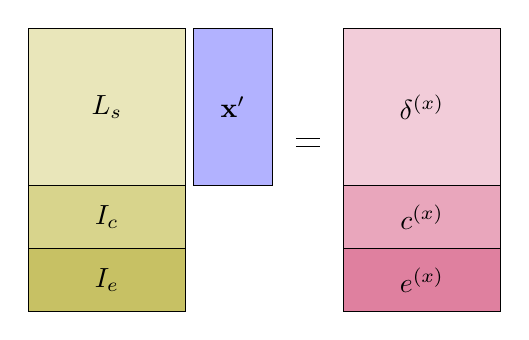
\begin{tikzpicture}
			\filldraw[fill=olive!20!white, draw=black] (0,0) rectangle node{$L_s$} (2,2);
			\filldraw[fill=olive!35!white, draw=black] (0,0) rectangle node{$I_c$} (2,-0.8);
			\filldraw[fill=olive!50!white, draw=black] (0,-0.8) rectangle node{$I_e$} (2,-1.6);
			\filldraw[fill=blue!30!white, draw=black] (2.1,0) rectangle node{$\mathbf{x'}$} (3.1,2);
			\draw (3.4, 0.50) -- (3.7, 0.50);
			\draw (3.4, 0.60) -- (3.7, 0.60);
			\filldraw[fill=purple!20!white, draw=black] (4,0) rectangle node{$\delta^{(x)}$} (6,2);
			\filldraw[fill=purple!35!white, draw=black] (4,0) rectangle node{$c^{(x)}$} (6,-0.8);
			\filldraw[fill=purple!50!white, draw=black] (4,-0.8) rectangle node{$e^{(x)}$} (6,-1.6);
		\end{tikzpicture}
		\end{center}
	\end{block}
	
\end{frame}

\begin{frame}
	\frametitle{{\bf \color{blue} Aplicações}}
	\framesubtitle{\color{blue} Edição de malhas}
	
	\begin{block}{\bf Edição - observações}
Como é utilizado o método dos mínimos quadrados para a resolução dos sistemas, talvez aconteça alguns erros de precisão.
		
		\medskip
		
Para minimizar estas falhas, após se encontrar a solução do sistema, pode-se forçar com que $v'_i = v_i$, para alguns $i$, para que pelo menos estes pontos não sofram erros de precisão;
	\end{block}
\end{frame}

\begin{frame}
	\frametitle{{\bf \color{blue} Aplicações}}
	\framesubtitle{\color{blue} Edição de malhas}
	
\begin{figure}[ht!]
	\centering
	\begin{subfigure}[b]{0.47\textwidth}
		\centering
		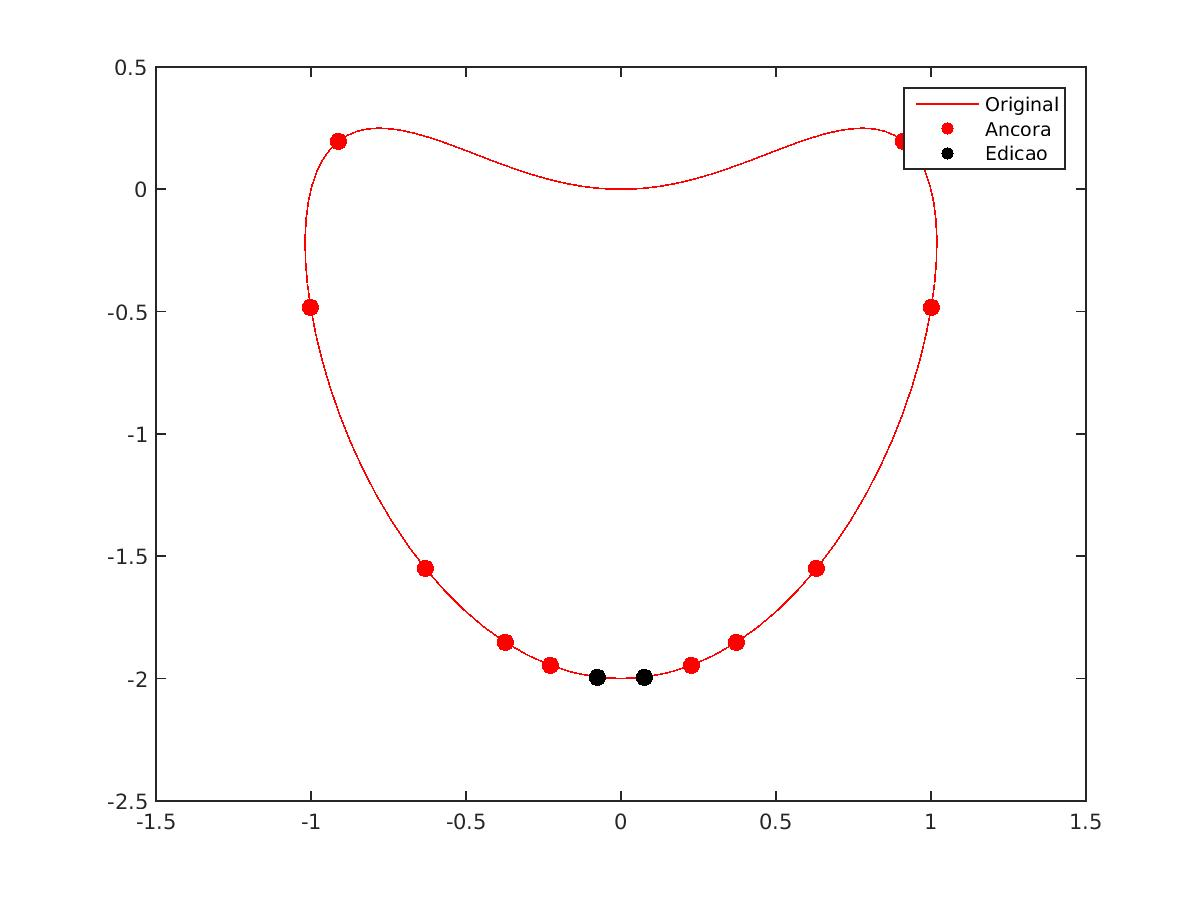
\includegraphics[trim={5cm, 2cm, 3cm, 2cm},clip,width=\textwidth]{imagens/malhaoriginal.jpg}
		\caption{Malha original}
		\label{fig:meshorigiedit}
	\end{subfigure}
	\hfill
	\begin{subfigure}[b]{0.47\textwidth}
		\centering
		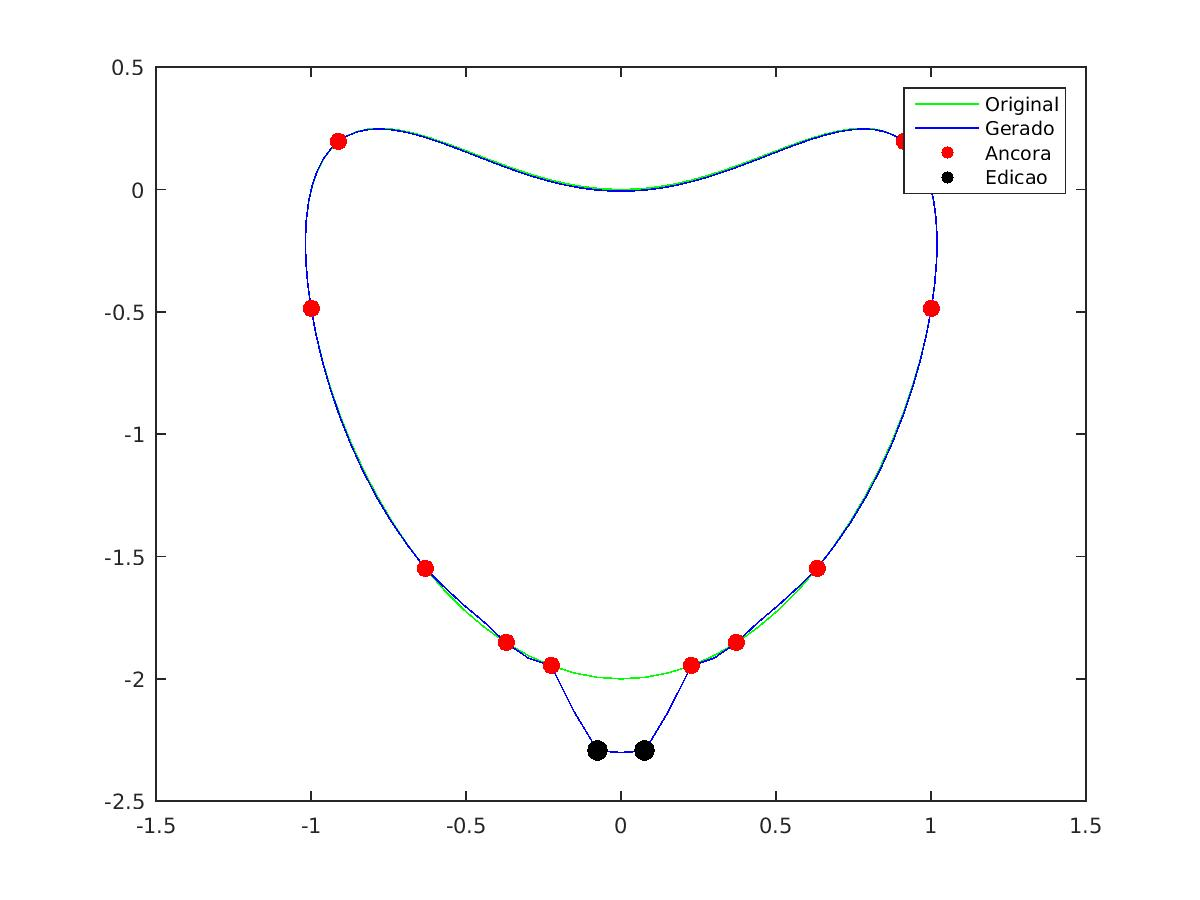
\includegraphics[trim={5cm, 2cm, 3cm, 2cm},clip,width=\textwidth]{imagens/malhaedicao.jpg}
		\caption{Malha editada}
		\label{fig:mesheditededit}
	\end{subfigure}
	\caption{Malha antes e após edição. Os pontos em vermelho são os pontos de âncora, e os pontos em preto são os editados.}
	\label{fig:editedmesh}
\end{figure}

\end{frame}